% VLDB template version of 2020-03-05 enhances the ACM template, version 1.7.0:
% https://www.acm.org/publications/proceedings-template
% The ACM Latex guide provides further information about the ACM template

\documentclass[sigconf, nonacm, balance=false, urlbreakonhyphens=true]{acmart}
\usepackage{amsmath, amsfonts, amsthm}
\usepackage{url}
\usepackage{makecell}
\usepackage{multirow}
\usepackage{longtable}
\usepackage{verbatim}
\usepackage{makecell}

% Allow URL Breakline
\def\UrlBreaks{\do\A\do\B\do\C\do\D\do\E\do\F\do\G\do\H\do\I\do\J
\do\K\do\L\do\M\do\N\do\O\do\P\do\Q\do\R\do\S\do\T\do\U\do\V
\do\W\do\X\do\Y\do\Z\do\[\do\\\do\]\do\^\do\_\do\`\do\a\do\b
\do\c\do\d\do\e\do\f\do\g\do\h\do\i\do\j\do\k\do\l\do\m\do\n
\do\o\do\p\do\q\do\r\do\s\do\t\do\u\do\v\do\w\do\x\do\y\do\z
\do\.\do\@\do\\\do\/\do\!\do\_\do\|\do\;\do\>\do\]\do\)\do\,
\do\?\do\'\do+\do\=\do\#}

\begin{document}
    \title{CS 130 Project 1: Threads\\Design Document}

    %%
    %% The "author" command and its associated commands are used to define the authors and their affiliations.
    \author{Tianyi Zhang}
    \affiliation{%
        \institution{School of Information Science and Technology}
        \state{2018533074}
    }
    \email{zhangty2@shanghaitech.edu.cn}

    \author{Haoran Dang}
    \affiliation{%
        \institution{School of Information Science and Technology}
        \state{2018533259}
    }
    \email{danghr@shanghaitech.edu.cn}

    \maketitle

    \setcounter{section}{-1}

    \section{Preliminaries}
        %%
        %% If you have any preliminary comments on your submission, notes for the
        %% TAs, or extra credit, please give them here.
        \subsection{Preliminary Comments}

        No preliminary comment for this project. 

        %%
        %% Please cite any offline or online sources you consulted while
        %% preparing your submission, other than the Pintos documentation, course
        %% text, lecture notes, and course staff.
        \subsection{References}
        
            \begin{itemize}
                \item \url{https://www.runoob.com/cprogramming/c-enum.html}: \\To understand \texttt{enum} in the code. 
            \end{itemize} 
    
    \section{Alarm Clock}
            
        \label{Alarm Clock}
    
        \subsection{Data Structures}
        
            \subsubsection{Copy here the declaration of each new or changed `\texttt{struct}' or `\texttt{struct}' member, global or static variable, `\texttt{typedef}', or enumeration. Identify the purpose of each in 25 words or less. } 
            
                \begin{itemize}
                    \item In file \texttt{threads/threads.h}
\begin{verbatim}
struct thread
{
  ...
  /* A counter of remaining sleeping ticks */
  int64_t sleeping_ticks;
  ...
}\end{verbatim}
                \end{itemize}
        
        \subsection{Algorithms}
        
            \subsubsection{Briefly describe what happens in a call to \texttt{timer\_sleep()}, including the effects of the timer interrupt handler. }
                When \texttt{timer\_slee\\p} is invoked, it set a counter inside the thread as a countdown of remaining sleeping ticks, and calls \texttt{thread\_block} to avoid it from running. In the counter, 0 stands for not sleeping and positive number stands for the remaining ticks.
            
                In each tick, timer interrupt is called, in which the total tick counters of the OS \texttt{ticks}, of the idle thread \texttt{idle\_ticks}, and of the kernel thread \texttt{kernel\_ticks} are updated. Then, the sleeping status of all threads is checked by calling \texttt{thread\_sleep\_monitor} through \texttt{thread\_foreach}, which will subtract the counter by 1 of all sleeping threads. When a counter reaches 0, its thread is unblocked by using \texttt{thread\_unblock}, which will put it into the ready list. 
            
            \subsubsection{What steps are taken to minimize the amount of time spent in the timer interrupt handler? } \label{Minimize timer interrupt handler}
                In the handler, only one operation
                \begin{verbatim}
thread_foreach (&thread_sleep_monitor, t);
                \end{verbatim}
                is added. Since Pintos does not maintain a list of sleeping items, and it is easy to check whether a thread is sleeping simply using \texttt{status} and \texttt{sleeping\_ticks}, it does not require much time even if we look into all the threads. 
        
        \subsection{Synchronization}
        
            \subsubsection{How are race conditions avoided when multiple threads call \texttt{timer\_sleep()} simultaneously? } \label{Race Conditions of Threads}
                Inspired by function \\\texttt{timer\_ticks}, we can use 
            \begin{verbatim}
enum intr_level old_level = intr_disable ();
...
intr_set_level (old_level);
\end{verbatim}
                to ensure a non-interruptible operation on the current thread. 
                
                First we call \texttt{intr\_disable}, which will make the process uninterruptible and returns the old status. Then we do our operations which are now uninterruptible. Finally, we restore the interrupt status by \texttt{intr\_set\_level}. 

                Thus, since the thread is uninterruptible, we can ensure the value of \texttt{sleeping\_ticks} is correct when the thread is blocked. 
            
            \subsubsection{How are race conditions avoided when a timer interrupt occurs during a call to \texttt{timer\_sleep()}? }
                Similar to \ref{Race Conditions of Threads}, all the operations in \texttt{timer\_sleep()} is uninterruptible, so the race condition of interrupts is avoided. 
        
        \subsection{Rationale}
            
            \subsubsection{Why did you choose this design? In what ways is it superior to another design you considered? }
                \texttt{thread\_foreach}, \texttt{thread\_block} and \texttt{thread\_unblock} is mentioned in the project guide, which are convenient to use to set or update the sleeping status of a thread.

                We considered using a special number like \texttt{-1} for threads which are not sleeping, and in each tick we unblock the threads whose \texttt{sleeping\_ticks} is 0. But such method requires more operations, and will cause one more cycle of sleep. 

                We also considered maintaining a list of sleeping threads, but as mentioned in \ref{Minimize timer interrupt handler}, it is costy to maintain an extra list when we can detect whether a thread is sleeping just by inspecting \texttt{status} and \texttt{sleeping\_ticks} of a thread. 
    
    \section{Priority Scheduling}

        \label{Priority Scheduling}

        \subsection{Data Structures}
            
            \subsubsection{Copy here the declaration of each new or changed `\texttt{struct}' or `\texttt{struct}' member, global or static variable, `\texttt{typedef}', or enumeration. Identify the purpose of each in 25 words or less. } 

                \begin{itemize}
                    \item In file \texttt{threads/threads.h}
\begin{verbatim}
struct thread
{
  ...
  /* List of holding locks. */
  struct list locks; 
  /* Priority without donation. */
  int priority_wo_donation;
  /* The lock a thread is waiting for. */
  struct lock *lock_wait;             
  ...
}
\end{verbatim}
                    \item In file \texttt{threads/synch.h}
\begin{verbatim}
struct lock
{
  ...
  /* Priority donated by this lock. */   
  int donated_priority;              
  ...
}
\end{verbatim}
                \end{itemize}

            \subsubsection{Explain the data structure used to track priority donation. Use ASCII art to diagram a nested donation.  (Alternately, submit a \texttt{.png} file.)}

                We use \texttt{lock* lock\_wait} to find the thread we are donating. And we store the locks held by the current thread in \texttt{thread.locks}. In the locks we store the priority donated by another thread which means we can find the max donated priority.
                \noindent \begin{figure}[H]
                    \centering
                    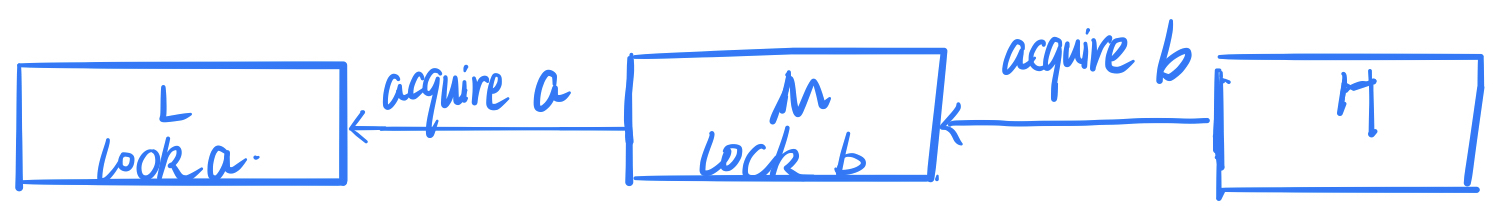
\includegraphics[width=25em]{pic.jpg}
                    \caption{Nested Donation}
                    \label{fig:my_label}
                \end{figure}

        \subsection{Algorithms}

            \subsubsection{How do you ensure that the highest priority thread waiting for a lock, semaphore, or condition variable wakes up first? } 
            
                We have already push all the blocked threads in the \texttt{sema.waiters} or \texttt{cond.waiters} when we block the threads. Therefore the only thing we need to do is sort the waiting list with the order of the thread's priority.Then the front element is the thread we want.

            \subsubsection{Describe the sequence of events when a call to \texttt{lock\_acquire()} causes a priority donation. How is nested donation handled? }

                When we call the \texttt{lock\_acquire()} we check whether the lock has a holder. Then we use the lock to locate its holder, update the holder's priority if the current thread's priority is higher. After that we will check the holder's \texttt{lock\_wait} then we can update the priority donated by holder if there is a thread holds a lock that holder wants to acquire. After doing the iterations, we will update the priority in a nested situation.

            \subsubsection{Describe the sequence of events when \texttt{lock\_release()} is called on a lock that a higher-priority thread is waiting for. }

                We will clear the \texttt{lock->holder} then reomove the lock from current thread's locks list. Then we call \texttt{thread\_update\_priority()} to update current thread's priority. Then we will use \texttt{sema\_down()} to unblock the thread which tried to acquire the lock, pop it from the waiting list. Then use \texttt{thread\_yield} to switch to the new thread. 

        \subsection{Synchronization}

            \subsubsection{Describe a potential race in \texttt{thread\_set\_priority()} and explain how your implementation avoids it.  Can you use a lock to avoid this race? }

                When we call \texttt{thread\_set\_priority()} to set a thread which has been donated by a higher priority, we cannot just change this thread's priority. We need to store the priority and then update to this priority after the donation.

                We just have a variable named \texttt{priority\_wo\_donation} to store the base priority. We just change this value if current thread is donated by another thread. And we cannot use a lock to avoid this race.

        \subsection{Rationale}

            \subsubsection{Why did you choose this design? In what ways is it superior to another design you considered? }

                We choose the design because we could use the \texttt{thread.locks} to get the highest priority donated by multiple threads easily. \texttt{thread.lock\_wait} enablesus to  find the thread we donate to. \texttt{lock.donated\_priority} will avoid the race for changing the priority of the current thread.

    \section{Advanced Scheduler}

        \label{Advanced Scheduler}

        \subsection{Data Structures}
            
            \subsubsection{Copy here the declaration of each new or changed `\texttt{struct}' or `\texttt{struct}' member, global or static variable, `\texttt{typedef}', or enumeration. Identify the purpose of each in 25 words or less. } 

                \begin{itemize}
                    \item In file \texttt{threads/threads.h}
\begin{verbatim}
...
/* Lowest "nice" value. */
#define NICE_MIN -20
/* Default "nice" value. */
#define NICE_DEFAULT 0
/* Highest "nice" value. */
#define NICE_MAX 20
...
struct thread
  {
    ...
    /* "nice" value of a thread */
    int nice;
    /* "recent_cpu" value of a thread */
    fixed_point recent_cpu;
    ...
  }\end{verbatim}
                    \item In file \texttt{threads/threads.c}
\begin{verbatim}
/* System load average */
fixed_point load_avg;\end{verbatim}
                \end{itemize}

        \subsection{Algorithms}

            \subsubsection{Suppose threads A, B, and C have nice values 0, 1, and 2. Each has a \texttt{recent\_cpu} value of 0. Fill in the table below showing the scheduling decision and the \texttt{priority} and \texttt{recent\_cpu} values for each thread after each given number of timer ticks:} 
                \begin{center}
                    \begin{tabular}{|c|c|c|c|c|c|c|c|}
                        \hline
                        \multirow{2}{*}{\makecell{Timer\\ticks}} & \multicolumn{3}{c|}{\texttt{recent\_cpu}} & \multicolumn{3}{c|}{\texttt{priority}} & \multirow{2}{*}{\makecell{Thread\\to run}} \\
                        \cline{2-7}
                        & A & B & C & A & B & C & \\
                        \hline
                        0 & 0 & 0 & 0 & 63 & 61 & 59 & A \\
                        \hline
                        4 & 4 & 0 & 0 & 62 & 61 & 59 & A \\
                        \hline
                        8 & 8 & 0 & 0 & 61 & 61 & 59 & B \\
                        \hline
                        12 & 8 & 4 & 0 & 61 & 60 & 59 & A \\
                        \hline
                        16 & 12 & 4 & 0 & 60 & 60 & 59 & B \\
                        \hline
                        20 & 12 & 8 & 0 & 60 & 59 & 59 & A \\
                        \hline
                        24 & 16 & 8 & 0 & 59 & 59 & 59 & C \\
                        \hline
                        28 & 16 & 8 & 4 & 59 & 59 & 58 & B \\
                        \hline
                        32 & 16 & 12 & 4 & 59 & 58 & 58 & A \\
                        \hline
                        36 & 20 & 12 & 4 & 58 & 58 & 58 & C \\
                        \hline
                    \end{tabular}
                \end{center}
            
            \subsubsection{Did any ambiguities in the scheduler specification make values in the table uncertain? If so, what rule did you use to resolve them? Does this match the behavior of your scheduler? }

            Yes, since the specification does not mention what the shceduler will do if the calculated priority of the two threads is the same. 

            Just as our implementation in task \ref{Alarm Clock} and \ref{Priority Scheduling}, the ready list is maintained as a priority list, and the sorting method will insert the item at the place after the items with same priority in the list. The value in this table uses the method similar to our implementation. 

            \subsubsection{How is the way you divided the cost of scheduling between code inside and outside interrupt context likely to affect performance? }

            Either when changing the \texttt{nice} by the thread itself or during an interrupt, the ready thread will be put into \texttt{ready\_list} according to the priority, so there seems to be small difference between these two situations in our implementation. 

        \subsection{Rationale}

            \subsubsection{Briefly critique your design, pointing out advantages and disadvantages in your design choices. If you were to have extra time to work on this part of the project, how might you choose to refine or improve your design? }

            \begin{enumerate}
                \item \textbf{Advantages:} Easy to implement and resource-saving, as it uses the original scheduler in task \ref{Priority Scheduling} and maintains only one list according to the calculated priority. 
                \item \textbf{Disadvantages:} The stability and performance of the scheduler still need to be improved. Also, complex scheduling algorithms considering not only calculated priority is not convenient to implement under this design. 
                \item \textbf{Things to do:} Figure out more about execution inside and outside interrupt context, and improve the stability by marking atomic operations, etc. 
            \end{enumerate}

            \subsubsection{The assignment explains arithmetic for fixed-point math in detail, but it leaves it open to you to implement it. Why did you decide to implement it the way you did? If you created an abstraction layer for fixed-point math, that is, an abstract data type and/or a set of functions or macros to manipulate fixed-point numbers, why did you do so? If not, why not?}

            Fixed-point numbers and opeartions are implemented in \texttt{threads/fixed-point.h} and \texttt{fixed-point.c}, in which we use a \texttt{struct}, containing only one \texttt{int} number, and a set of function. 
            
            Although (maybe) not all the functions are used, implementing it will reduce the workload afterwards and will make the code neat than directly showing a lot of computation processes. Meanwhile, using a \texttt{struct} instead of \texttt{typedef int fixed\_point} can directly show misuse of the types in the compiler, so that we don't need to worry about wrong type conversion. 
    
    \section{Survey Questions}

        \subsubsection*{In your opinion, was this assignment, or any one of the three problems in it, too easy or too hard? Did it take too long or too little time? }

            Tasks in project 1 are not quite "hard" yet but it does require a lot of time since the operating system is a complex task. 

        \subsubsection*{Did you find that working on a particular part of the assignment gave you greater insight into some aspect of OS design? }

            Working on \texttt{timer\_sleep} and \texttt{timer\_interrupt} in task \ref{Alarm Clock} and \ref{Advanced Scheduler} offers us a direct impression on what happens when CPU ticks. Meanwhile, in \ref{Priority Scheduling} we considered a lot of different situations, which inspires us to understand how nested changes take place in the operating system. 

        \subsubsection*{Is there some particular fact or hint we should give students in future quarters to help them solve the problems? Conversely, did you find any of our guidance to be misleading? }

            Actually no. But I guess it would be slightly better if the TAs can introduce some Git GUI softwares as they can increase the efficiency when using complex functions sometimes. 

        \subsubsection*{Do you have any suggestions for the TAs to more effectively assist students, either for future quarters or the remaining projects? }

            Not yet. 

        \subsubsection*{Any other comments? }

            Not yet. 
    
    \section*{Contributors}

        \begin{center}
            \begin{tabular}{|c|c|c|c|}
                \hline
                \multicolumn{2}{|c|}{Task} & \makecell{Tianyi\\Zhang} & \makecell{Haoran\\Dang} \\
                \hline
                \multirow{4}{*}{\makecell{Task \ref{Alarm Clock} \\ Alarm Clock}} 
                    & Concept & \checkmark & \checkmark \\
                    \cline{2-4}
                    & Implementation & \checkmark & \checkmark \\
                    \cline{2-4}
                    & Debugging & \checkmark & \checkmark \\
                    \cline{2-4}
                    & Design Document & & \checkmark \\
                \hline
                \multirow{4}{*}{\makecell{Task \ref{Priority Scheduling} \\ Priority Scheduling}} 
                    & Concept & \checkmark & \checkmark \\
                    \cline{2-4}
                    & Implementation & \checkmark & \checkmark \\
                    \cline{2-4}
                    & Debugging & \checkmark & \\
                    \cline{2-4}
                    & Design Document & \checkmark & \\
                \hline
                \multirow{4}{*}{\makecell{Task \ref{Advanced Scheduler} \\ Advanced Scheduler}} 
                    & Concept & \checkmark & \checkmark \\
                    \cline{2-4}
                    & Implementation & \checkmark & \checkmark \\
                    \cline{2-4}
                    & Debugging & \checkmark & \checkmark \\
                    \cline{2-4}
                    & Design Document & & \checkmark \\
                \hline
            \end{tabular}
        \end{center}

\end{document}
\endinput
